\selectlanguage{ngerman}%
\frenchspacing%
\begin{ledgroupsized}[r]{120mm}%
\footnotesize%
\pstart%
\noindent\textbf{Überlieferung:}%
\pend%
\end{ledgroupsized}%
\begin{ledgroupsized}[r]{114mm}%
\footnotesize%
\pstart%
\parindent -6mm%
\makebox[6mm][l]{\textit{L}}%
\pagelabel{LH_35_11_14_005-006_ueberlieferung}%
Aufzeichnung:
LH~XXXV~11,\;14 Bl.\;5\textendash6.
Ein Bogen~4\textsuperscript{o};
\href{\Scan{LH_35_11_14_005-006wz}}{Wasserzeichen} im Falz.
Vier Seiten. %
Ein Kustos am Ende von Bl.\;6\,v\textsuperscript{o} verweist auf die \textit{Scheda 2} (N.\;\ref{58939}).%
\pend%
\end{ledgroupsized}%
\selectlanguage{latin}%
\frenchspacing%
\vspace{8mm}%
\pstart%
\normalsize%
\noindent%
\lbrack%
\href{\Scan{LH_35_11_14_005r}}%
{5\,r\textsuperscript{o}}%
\rbrack%
\hfill%
\raggedleft%
31.\;Octob.\;1690
\pend%
\pstart%
\centering%
De impulsu Eccentrico sched. 1%
\indexS{impulsus eccentricus}%
\indexS{scheda}
\pend
\vspace{0.5em}
\pstart%
\noindent%
\edlabel{LH_35_11_14_005-006_005r_methodus-1}%
\edtext{Ad eccentricos corporum incursus%
\indexS{incursus eccentricus}%
\indexS{corpus incurrens}%
}{%
\lemma{Ad}\Bfootnote{%
\textit{(1)}~obliquos co
\textit{(2)}~eccentricos corporum incursus%
~\textit{L}}}
explicandos considerandum est lateralia,%
\indexS{corpus laterale}
quae non per se impelluntur,
ab ipsis per se impulsis quodammodo trahi.
Ut si
globus \textit{A}%
\indexS{globus incurrens}
centrice incurrat in globum \textit{B},%
\indexS{incursus centricus}
sed globo \textit{B} alligatus sit globus \textit{C},%
\indexS{globus alligatus}
tunc impelletur quidem globus\;\textit{B},
sed a globo \textit{B} impulso%
\indexS{globus impulsus}
trahetur globus \textit{C}.%
\indexS{globus tractus}
Atque ita efficitur
ut eccentrice impulsum intelligatur totum compositum \textit{BC}.%
\indexS{corpus impulsum eccentrice}%
\indexS{corpus compositum}%
\edlabel{LH_35_11_14_005-006_005r_methodus-2}%
\pend%
\vspace{1.25em}%
\centerline{%
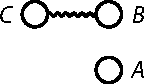
\includegraphics[width=0.16\textwidth]{gesamttex/edit_VIII-4/images/LH_35_11_14_005-006_d01_005r.pdf}}%
\vspace{0.25em}%
\centerline{%
\lbrack\textit{Fig.\:1}\rbrack}%
\vspace{1.0em}%
\pstart%
\noindent%
Antequam ergo impulsus%
\indexS{impulsus eccentricus}
tractionibus conjungamus,%
\indexS{impulsus conjunctus tractioni}
ipsas tractiones consideremus per se.%
\indexS{tractio conjuncta impulsui}
Licet enim omnis tractio per consequentiam%
\indexS{consequentia}
et ipsa ad impulsum%
\indexS{impulsus eccentricus}
redigatur,
id tamen nunc considerari necesse non est,
sufficitque assumi corporum connexionem atque tractionem%
\indexS{tractio conjuncta impulsui}%
\lbrack,\rbrack\
quaecunque demum sit causa%
\indexS{causa firmitatis}
quae fili trahentis%
\indexS{filum trahens}
\edtext{alteriusve vinculi%
\indexS{vinculum rigidum}%
}{%
\lemma{alteriusve}\Bfootnote{%
vinculi
\textit{erg.\;L}}}
firmitatem facit.%
\indexS{firmitas fili}%
\indexS{firmitas vinculi}
\pend%
\pstart%
\edtext{Ponamus ergo
\edtext{globum \textit{B}%
\indexS{globus incurrens}%
}{%
\lemma{globum \textit{B}}\Cfootnote{%
Vgl. das Diagramm \lbrack\textit{Fig.\:2}\rbrack.
Das Band ist dort nicht als \textit{D} bezeichnet.%
}}
initio solum esse in motu,%
\indexS{motus globi}
quiescente \textit{C},%
}{\lemma{Ponamus}\Bfootnote{%
\textit{(1)}~\bars{esse \textit{streicht Hrsg.}}
\textit{(2)}~ergo
\textit{(a)}~filum
\textit{(b)}~globum \textit{B} initio
\textit{(aa)}~esse in motu, solum quiescente \textit{C}
\textit{(bb)}~solum esse %
\lbrack...\rbrack\ quiescente \textit{C},%
~\textit{L}}}
ipsum autem \textit{B} progredientem induere
\edtext{se in retia vinculi%
\indexS{retia vinculi}%
\indexS{vinculum rigidum}%
}{%
\lemma{se}\Bfootnote{%
\textit{(1)}~in vincula
\textit{(2)}~in retia vinculi%
~\textit{L}}}
\textit{D} connexi globo \textit{C},%
\indexS{globi connexi}
et ita a globo \textit{C}
velut visco%
\indexS{viscus}
quodam capi,
quaeritur
quis oriatur motus compositi ex ambobus?%
\indexS{motus compositi} %
\edtext{Is determinatus habebitur ex solitis principiis nostris%
\indexS{principium nostrum}%
}{%
\lemma{Is}\Bfootnote{%
\textit{(1)}~ex sequentibus principibus
\bars{erit \textit{streicht Hrsg.}}
\textit{(2)}~determinatus habebitur %
\lbrack...\rbrack\ principiis nostris,%
~\textit{L}}}%
\lbrack:\rbrack\
nam centrum gravitatis commune%
\indexS{centrum gravitatis commune}
eandem debet habere celeritatem%
\indexS{celeritas centri gravitatis}
quam ante et in easdem partes,
ut eadem maneat vis directrix%
\indexS{vis directrix}%
\lbrack;\rbrack\
deinde oportet eandem quoque
\edtext{manere}{%
\lemma{manere}\Bfootnote{%
\textit{erg.\;L}}}
vim respectivam,%
\indexS{vis respectiva}
seu corporum
\edtext{\lbrack\textit{B}\rbrack\
et
\lbrack\textit{C}\rbrack}{%
\lemma{\textit{A}}\Bfootnote{%
et \textit{B}
\textit{L~ändert Hrsg.}}}
accedendi
recedendique a se invicem conatum.%
\indexS{conatus accedendi}%
\indexS{conatus recedendi}
Unde eadem quoque manebit vis absoluta.%
\indexS{vis absoluta}
\edlabel{35_11_14_005-006_3a}%
\edtext{}{%
\xxref{35_11_14_005-006_3a}{35_11_14_005-006_3b}%
\lemma{absoluta}\Bfootnote{%
\textit{(1)}~Et prim \lbrack/\rbrack\
\textit{(2)}~At
\textit{(3)}~Ac primum ponamus
\textit{(a)}~corpora esse aequalia
\textit{(b)}~globos esse aequales,%
~\textit{L}}}%
\pend%
\pstart%
\edlabel{LH_35_11_14_005-006_005r_cntrgyr-1}%
Ac primum ponamus globos%
\indexS{globus incurrens}%
\indexS{globi connexi}
esse aequales,%
\edlabel{35_11_14_005-006_3b}
et
\edtext{proinde}{%
\lemma{proinde}\Bfootnote{%
\textit{erg.\;L}}}
centrum gravitatis \textit{G} esse in medio,%
\indexS{centrum gravitatis commune}
viamque ejus%
\indexS{via centri gravitatis}
\edtext{\textit{\ind{1}G\ind{2}G}.
Haec}{%
\lemma{\textit{\ind{1}G\ind{2}G}}\Bfootnote{%
\textit{(1)}~quae
\textit{(2)}~. Haec%
~\textit{L}}}
continuetur recta in \textit{\ind{3}G},
sic ut recta
\edtext{\lbrack\textit{\ind{1}G}\ind{3}\textit{G}\rbrack%
}{%
\lemma{\textit{\ind{1}G\ind{2}G}}\Bfootnote{%
\textit{L~ändert Hrsg.}}}
sit dupla rectae \textit{\ind{1}G\ind{2}G}
vel \textit{\ind{2}G\ind{3}G}.
\edtext{Deinde vinculum globorum%
\indexS{globi connexi}
sit rigidum%
\indexS{vinculum rigidum}%
\lbrack,\rbrack\
quod ponamus consistere in linea rigida
centra connectente,%
\indexS{linea rigida}%
\indexS{linea connectens centra}
normali ad lineam motus%
\indexS{linea motus}%
\lbrack;\rbrack\
necesse}{%
\lemma{Deinde}\Bfootnote{%
\textit{(1)}~si ponamus
\textit{(2)}~vinculum globorum sit rigidum
\bars{quod ponamus \lbrack...\rbrack\ lineam motus \textit{erg.}}
necesse%
~\textit{L}}}
est globos%
\indexS{globi connexi}
a se recedere conantes%
\lbrack,\rbrack\
moveri circa aliquod rigidae%
\indexS{linea rigida}
\edtext{seu inflexilis%
\indexS{linea inflexilis}%
}{%
\lemma{seu}\Bfootnote{%
inflexilis
\textit{erg.\;L}}}
lineae \textit{C\ind{ 2}B} punctum %
tanquam centrum.%
\indexS{centrum gyrationis}
Vis autem%
\indexS{vis respectiva}
\edtext{respectiva eadem est}{%
\lemma{respectiva}\Bfootnote{%
\textit{(1)}~perinde
\textit{(2)}~eadem est%
~\textit{L}}}
ac si corpora \textit{B} et \textit{C} celeritate
\edtext{mo\lbrack l\rbrack ibus}{%
\lemma{motibus}\Bfootnote{\textit{L~ändert Hrsg.}}}
reciproca%
\indexS{celeritas reciproca moli}
sibi occurrerent%
\indexS{corpora occurrentia sibi}
et \textit{B} tenderet
\edtext{celeritate \textit{\ind{ 2}BL}%
}{\lemma{celeritate \textit{\ind{ 2}BL}}\Cfootnote{%
Vgl. das Diagramm \lbrack\textit{Fig.\:3}\rbrack.%
}}
et \textit{C} celeritate \textit{CM},
ita ut esset \textit{BL} ad \textit{CM} %
ut \textit{C} ad \textit{B}.
Quodsi igitur aequales sunt globi,%
\indexS{globus incurrens}%
\indexS{globi connexi}
erunt et celeritates \textit{BL},
\textit{CM} aequales,
quod fiet si gyrentur circa punctum medium,%
\indexS{gyratio circa punctum medium}
id est circa centrum gravitatis%
\indexS{centrum gravitatis commune}%
\indexS{gyratio circa centrum gravitatis}
\edlabel{LH_35_11_14_005r_hdsum-1}%
\textit{\ind{2}G}.
Quae celeritates conatusve%
\indexS{conatus procedendi recta}
recta procedendi,
nunc ob vinculum%
\indexS{vinculum rigidum}
in gyrationem%
\indexS{celeritas versa in gyrationem}%
\indexS{conatus versus in gyrationem}
vertentur;
quod ut fiat
eodem servato celeritatis gradu%
\indexS{gradus celeritatis servatus}%
\lbrack,\rbrack\
circulatio fit circa punctum medium \textit{\ind{2}G}%
\indexS{circulatio circa punctum medium}
quod simul est centrum gravitatis.%
\indexS{centrum gravitatis commune}%
\indexS{circulatio circa centrum gravitatis}%
\edtext{}{%
\xxref{LH_35_11_14_005r_hdsum-1}{LH_35_11_14_005r_hdsum-2}%
\lemma{gravitatis}\Bfootnote{%
\textit{\ind{2}G}.
\textit{(1)}~Quid
\textit{(2)}~Si corpora \textit{B} et \textit{C} ponantur inaequalia nihilominus gyratio fiet circa centrum gravitatis \textit{\ind{2}G}{,} nam ut
\textit{(a)}~gyrat
\textit{(b)}~celeritas
\textit{(3)}~Quae celeritates 
\textit{(a)}~in gyratione
\textit{(b)}~conatusve recta procedendi,
\bars{nunc \textit{erg.}}
ob vinculum 
\lbrack...\rbrack\
ut in gyratione
\bars{circa punctum ut \textit{G} \textit{erg.}}
eadem servetur celeritas,%
~\textit{L}}}%
\pend%
\pstart%
Si corpora \textit{B} et \textit{C} ponantur inaequalia,
nihilominus fiet gyratio circa centrum gravitatis,
nam ut in gyratione%
\indexS{gyratio circa centrum gravitatis}
circa punctum ut \textit{G}
eadem servetur celeritas,%
\indexS{celeritas servata in gyratione}%
\edlabel{LH_35_11_14_005r_hdsum-2}
quae erat conatus recti,
oportet esse \textit{BG} ad \textit{CG}
ut \textit{BL} ad
\edtext{\lbrack\textit{CM}\rbrack,}{%
\lemma{\textit{CL}}\Bfootnote{%
\textit{L~ändert Hrsg.}}}
id est ut \textit{C} ad \textit{B}.
Itaque \textit{G} est centrum gravitatis.%
\indexS{centrum gravitatis commune}%
\edlabel{LH_35_11_14_005-006_005r_cntrgyr-2}%
\pend%
\vspace{1.50em}%
\centerline{%
\hspace*{-50mm}%
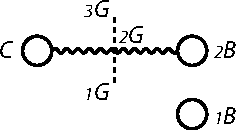
\includegraphics[width=0.25\textwidth]{gesamttex/edit_VIII-4/images/LH_35_11_14_005-006_d02_005r.pdf}}%
\vspace{0.25em}%
\centerline{%
\hspace*{-50mm}%
\lbrack\textit{Fig.\:2}\rbrack}%
\vspace{-8.40em}%
\centerline{%
\hspace*{50mm}
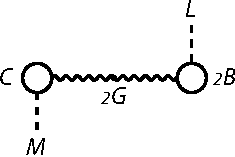
\includegraphics[width=0.26\textwidth]{gesamttex/edit_VIII-4/images/LH_35_11_14_005-006_d03_005r.pdf}}%
\vspace{0.0em}%
\centerline{%
\hspace*{50mm}%
\lbrack\textit{Fig.\:3}\rbrack}%
\newpage%
\pstart%
Itaque perinde movebuntur duo corpora%
\indexS{corpora connexa}
post connexionem%
\indexS{connexio corporum}
ac si habuissent motum communem centri gravitatis,%
\indexS{motus communis centri gravitatis}%
\indexS{centrum gravitatis}
quem et retinebunt,%
\indexS{motus retentus}
proprium autem,%
\indexS{motus proprius}
qui demto communi%
\indexS{motus communis demtus}
\edtext{sequitur,
in gyrum}{%
\lemma{sequitur,}\Bfootnote{%
\bars{quem \textit{streicht Hrsg.}}
in gyrum%
~\textit{L}}}
convertent.%
\indexS{motus conversus in gyrum}%
\indexS{gyrus post incursum}
\lbrack%
\href{\Scan{LH_35_11_14_005v}}%
{5\,v\textsuperscript{o}}%
\rbrack%
\pend%
\pstart%
Eadem vera sunt,
si ambo corpora sint in motu,%
\indexS{corpora occurrentia sibi}
sed parallelas lineas%
\indexS{linea motus}
\lbrack(\protect\vphantom)\rbrack%
ad lineam vinculi%
\indexS{linea vinculi}%
\indexS{vinculum normale ad lineam motus}
scilicet normales%
\lbrack\protect\vphantom()\rbrack\
motu describant.
\pend%
\pstart%
Sed quid
si vinculum ad lineam%
\indexS{linea motus}
\edtext{motus sit obliquum?%
\indexS{vinculum obliquum ad lineam motus}
Omisso}{%
\lemma{motus}\Bfootnote{%
\textit{(1)}~\textlangle motus\textrangle\
\textit{(2)}~sit obliquum
\textit{(a)}~; ut omisso
\textit{(b)}~? Omisso%
~\textit{L}}}
motu communi%
\indexS{motus communis}
\edtext{centri gravitatis%
\indexS{motus centri gravitatis}%
\indexS{centrum gravitatis commune}%
}{%
\lemma{centri}\Bfootnote{%
gravitatis
\textit{erg.\;L}}}
consideremus proprium%
\indexS{motus proprius}
\edtext{utriusque reciprocumque%
\indexS{motus reciprocus}%
}{%
\lemma{utriusque}\Bfootnote{%
reciprocumque
\textit{erg.\;L}}}
tantum%
\lbrack,\rbrack\
in quo consistit vis respectiva.%
\indexS{vis respectiva}
\edtext{%
Is componi intelligetur ex duobus%
\indexS{motus compositus}%
\lbrack,\rbrack\
uno normali ad
\edtext{vinculum \textit{CB},}{%
\lemma{vinculum \textit{CB}}\Cfootnote{%
Vgl. das Diagramm \lbrack\textit{Fig.\:4}\rbrack.}}%
\indexS{motus normalis ad vinculum}
altero parallelo,%
\indexS{motus parallelus ad vinculum}
et normalis quidem transferetur in gyrationem,%
\indexS{gyratio post incursum}%
\indexS{motus translatus in gyrationem}
sed parallelus pariet distractionem vinculi%
\indexS{distractio vinculi}%
\indexS{vinculum rigidum}
\edtext{si ejus sit capax,}{%
\lemma{si}\Bfootnote{%
ejus sit capax
\textit{erg.\;L}}}
cum secundum ipsum corpora \textit{C}
et \textit{\ind{2}B}
reciprocis celeritatibus in diversa trahant.%
\indexS{celeritas reciproca}%
\indexS{corpora trahentia in diversa}
Itaque is motus erit perditus pro toto.%
\indexS{motus perditus}
Itaque hic quoque casus est resolutus.%
\indexS{casus resolutus}%
}%
{\lemma{\textit{Am Rand:}}%
\Afootnote{Hinc
si explicatum esset
si \textit{A} incurreret in \textit{B}%
\indexS{incursus eccentricus}
angulo ad \textit{BC} recto%
\indexS{angulus incursus rectus}%
\lbrack,\rbrack\
explicatum etiam esset
quid in obliquo%
\indexS{angulus incursus obliquus}%
\lbrack:\rbrack\
nam eatenus ictus parallelus%
\indexS{ictus parallelus}
haberetur pro centrico.%
\indexS{ictus centricus}%
}}
Et quidem compositio haec motuum%
\indexS{compositio motuum}
cum fiat salva potentiae quantitate,%
\indexS{quantitas potentiae}%
\indexS{potentia salva}
cum summa quadratorum sit eadem,%
\indexS{summa quadratorum}
tute a nobis introducitur.
\pend%
\pstart%
Si
\edtext{vinculum esset omni rigore destitutum,%
\indexS{vinculum flexile}
simpliciterque flexile,}{%
\lemma{vinculum}\Bfootnote{%
\textit{(1)}~non esset rigidum
\textit{(2)}~esset omni \lbrack...\rbrack\ simpliciterque flexile,%
~\textit{L}}}
nulla fieret gyratio%
\indexS{gyratio nulla}
sed
\edtext{tantum}{%
\lemma{tantum}\Bfootnote{%
\textit{erg.\;L}}}
tractio,%
\indexS{tractio post occursum}
adeoque tota vis respectiva%
\indexS{vis respectiva}
\edtext{in vinculi Elastro%
\indexS{elastrum vinculi}%
}{\lemma{in}\Bfootnote{%
\textit{(1)}~vinculo
\textit{(2)}~vinculi Elastro%
~\textit{L~}}}
consumeretur.%
\indexS{vis consumta in elastrum}
\pend%
\vspace{1.25em}%
\centerline{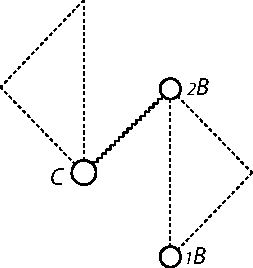
\includegraphics[width=0.26\textwidth]{gesamttex/edit_VIII-4/images/LH_35_11_14_005-006_d04_005v.pdf}}
\vspace{0.25em}
\centerline{\lbrack\textit{Fig.\:4}\rbrack}%
\newpage%
\pstart%
Nunc transferamus ista ad concursum,%
\indexS{concursus corporum}
\edtext{redeamusque ad
\edtext{tres globos%
\indexS{globus incurrens}%
\indexS{globi connexi}
\textit{A},\,\textit{B},\,\textit{C},%
}{\lemma{tres globos \textit{A},\,\textit{B},\,\textit{C}}\Cfootnote{%
Vgl. das Diagramm \lbrack\textit{Fig.\:5}\rbrack.}}%
}{\lemma{redeamusque}\Bfootnote{%
ad
\textit{(1)}~tria corpora
\textit{(2)}~tres globos \textit{A},\,\textit{B},\,\textit{C},%
~\textit{L}}}
et ponamus \textit{A} incurrere in \textit{B}
connexum cum \textit{C} vinculo inflexili.%
\indexS{vinculum inflexile}%
\indexS{globus incurrens}%
\indexS{globi connexi}
\edtext{\lbrack An}{%
\lemma{\lbrack An}\Cfootnote{%
Eckige Klammer von Leibniz.}}
perinde erit
ac si\;\textit{B} tantillum remotum esset a vinculo%
\indexS{vinculum inflexile}
\edtext{in momento concursus%
\indexS{momentum concursus}%
}{%
\lemma{in}\Bfootnote{%
momento concursus
\textit{erg.\;L}}}
et mox statim in ipsum
\edtext{indueretur?%
\indexS{globus indutus in vinculum}
Ita enim}{\lemma{indueretur}\Bfootnote{%
\textit{(1)}~, nam
\textit{(2)}~?
\textit{(a)}~Itaque
\textit{(b)}~Ita enim%
~\textit{L}}}
perinde \textit{A} reflectetur%
\indexS{globus reflexus}
ac si \textit{B} esset solum,
et \textit{B} deinde pergens motu %
quem
\edtext{ex legibus concursus centrici notis}{%
\lemma{ex le\-gi\-bus \lbrack...\rbrack\ notis}%
\Cfootnote{%
Siehe etwa G.\,W. \textsc{Leibniz},
\textit{Leges concursuum}
(\textit{LSB} VIII,\;3 N.\;67);\cite{01383}
\textit{Dynamica}, pars II, sectio III, prop.\;1\textendash15
(%
\textit{CFP}~I, S.\;392--417~\bracks{A};
II.2, S.\;490--518~\bracks{C}).\cite{01354}%
}}
acceperat%
\indexS{lex concursus centrici}%
\indexS{motus acceptus}
seque in vinculum induens%
\indexS{globus indutus in vinculum}
efficiet
quod paulo ante proposuimus.
Idque rationi%
\indexS{consentaneum rationi}
\edtext{consentaneum putes,}{%
\lemma{consentaneum}\Bfootnote{%
\textit{(1)}~est,
\textit{(2)}~putes,%
~\textit{L}}}
quorum
\edtext{enim}{%
\lemma{enim}\Bfootnote{%
\textit{erg.\;L}}}
unum in alterum desinit,
eorum et effectus sibi accedere%
\indexS{effectus accedens}
atque in se invicem
\edtext{tandem}{%
\lemma{tandem}\Bfootnote{%
\textit{erg.\;L}}}
desinere
\edtext{\lbrack debent\rbrack.}{%
\lemma{debeant}\Bfootnote{%
\textit{L~ändert Hrsg.}}}
Jam Hypothesis%
\indexS{hypothesis}
\textit{B} vinculo jam appositi%
\indexS{globus appositus vinculo}
et Hypothesis%
\indexS{hypothesis}
ejusdem a vinculo tantillum remoti,%
\indexS{globus remotus a vinculo}
sunt duo status quantumlibet exigue differentes.%
\indexS{status differens}
Verum sciendum est
\edtext{id in}{%
\lemma{id}\Bfootnote{%
in
\bars{in \textit{streicht Hrsg.}}
simplicibus%
~\textit{L}}}
simplicibus locum habere,
hic vero non aeque.
Et
\edtext{nec in centricis concursibus%
\indexS{concursus centricus}%
}{%
\lemma{nec}\Bfootnote{%
in
\textit{(1)}~communi
\textit{(2)}~centricis concursibus%
~\textit{L}}}
succedere,
multum enim interest exempli causa,
utrum
\edtext{\textit{L} incurrat in \textit{M}%
}{%
\lemma{\textit{L} incurrat in \textit{M}}\Cfootnote{%
Vgl. das Diagramm \lbrack\textit{Fig.\:6}\rbrack.}}
compositum cum \textit{N},%
\indexS{corpus compositum}
an vero ab eo nonnihil remotum,
quanquam certo comparandi modo semper effectus sibi%
\indexS{effectus accedens}
\edtext{accedant.
\edtext{%
Nec semper in compositis%
\indexS{corpus compositum}
locum habet processus per gradus,%
\indexS{processus per gradus}
nisi certo modo intellectus;%
}{%
\lemma{\textit{Am Rand:}}%
\Afootnote{NB Fortasse locum habent quae rejecimus.%
}}
sic refractiones subito transiliunt in reflexiones%
\indexS{refractio transiliens in reflexionem}%
\indexS{reflexio orta e refractione}
ubi ad certam obliquitatem%
\indexS{obliquitas incursus}
perventum est.%
}{\lemma{accedant.}\Bfootnote{%
\textit{(1)}~Sic et in refractionibus, ubi ad
\textit{(2)}~Nec semper \lbrack...\rbrack\ refractiones subito
\textit{(a)}~dissiliunt
\textit{(b)}~transiliunt in %
\lbrack...\rbrack\ perventum est.%
~\textit{L}}}
Itaque sic potius
\edtext{procedendum:\rbrack}{%
\lemma{procedendum:\rbrack\,}\Cfootnote{%
Eckige Klammer von Leibniz.}}%

\pend%
\vspace{2.5em}%
\centerline{\hspace{-95mm}%
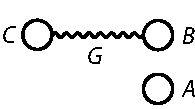
\includegraphics[width=0.20\textwidth]{gesamttex/edit_VIII-4/images/LH_35_11_14_005-006_d05_005v.pdf}}%
\vspace{0.0em}%
\centerline{\hspace{-95mm}%
\lbrack\textit{Fig.\:5}\rbrack}%
\vspace{-6.0em}%
\centerline{%
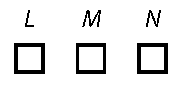
\includegraphics[width=0.20\textwidth]{gesamttex/edit_VIII-4/images/LH_35_11_14_005-006_d06_005v.pdf}}%
\vspace{0.5em}%
\centerline{%
\lbrack\textit{Fig.\:6}\rbrack}%
\vspace{-5.25em}%
\centerline{\hspace{95mm}%
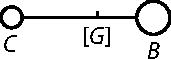
\includegraphics[width=0.18\textwidth]{gesamttex/edit_VIII-4/images/LH_35_11_14_005-006_d07_005v.pdf}}%
\vspace{1.0em}%
\centerline{\hspace{95mm}%
\lbrack\textit{Fig.\:7}\rbrack}%
\newpage%
\pstart%
\edlabel{LH_35_11_14_005-006_005v_navis-1}%
Corpora \textit{B} et \textit{C}%
\indexS{corpora connexa}
vinculo rigido connexa%
\indexS{vinculum rigidum}
concurrere intelligentur cum \textit{A},
et ita quidem ut ferri intelligantur motu communi centri gravitatis,%
\indexS{motus communis}%
\indexS{motus centri gravitatis}%
\indexS{centrum gravitatis commune}
velut in navi,%
\indexS{navis}
et motu proprio reciproco,%
\indexS{motus proprius}%
\indexS{motus reciprocus}
ita ut sit celeritas \textit{A} ad celeritatem \textit{B, C}
ut $B + C$ est ad \textit{A}.%
\edlabel{LH_35_11_14_005-006_005v_navis-2}
Jam ubi \textit{A} incurrit in \textit{B}, %
considerandum est%
\lbrack:\rbrack\
quatenus \textit{B} et \textit{C} gyrare debent
circa aliquod centrum,%
\indexS{gyratio circa centrum}
eatenus perinde
\edtext{e\lbrack st\rbrack}{%
\lemma{e}\Bfootnote{%
\textit{L~ändert Hrsg.}}}
ac si \textit{B} et \textit{C} pariter centrice impellerentur%
\indexS{corpus impulsum centrice}%
\indexS{impulsus centricus}
\edtext{tantum%
\lbrack,\rbrack\
\edtext{corpus oppositum \textit{C}%
}{\lemma{corpus oppositum \textit{C}}\Cfootnote{%
Vgl. das Diagramm \lbrack\textit{Fig.\:7}\rbrack.}}
sumendo tanquam tanto
\edtext{m\lbrack in\rbrack us,}{%
\lemma{m\lbrack in\rbrack us}\Cfootnote{%
Ist \textit{G} gemeinsamer Schwerpunkt der Körper \textit{B} und \textit{C}, so gilt $B : GC = C : GB.$}}
quanto%
}{%
\lemma{tantum}\Bfootnote{%
\textit{(1)}~considerando
\textit{(a)}~\bars{oppositum \textit{erg.}}
\textit{C} velut tanto m
\textit{(b)}~oppositum
\textit{(2)}~corpus oppositum \textit{C} sumendo tanquam
\bars{tanto \textit{erg.}}
\bars{majus \textit{ändert Hrsg.}},
quanto%
~\textit{L}}}
est a centro remotius.%
\indexS{centrum gyrationis}
Punctum autem istud\;\textit{G} est ipsum centrum gravitatis%
\indexS{centrum gravitatis commune}
corporum \textit{B} et \textit{C},
itaque perinde sic fiet
ac si \textit{B} esset duplum.
\lbrack%
\href{\Scan{LH_35_11_14_006r}}%
{6\,r\textsuperscript{o}}%
\rbrack%
\pend%
\pstart%
Videamus
an exitus inde habeatur%
\indexS{exitus}
\edtext{quod%
\lbrack,\rbrack\
dividendo}{%
\lemma{quod}\Bfootnote{%
\bars{quidem \textit{gestr.}}
dividendo%
~\textit{L}}}
corpora utcunque%
\lbrack,\rbrack\
eadem in ipsis manet vis respectiva%
\indexS{vis respectiva}%
\lbrack;\rbrack\
non tantum ergo debet servari
\edtext{eadem vis respectiva%
\indexS{vis respectiva}
inter}{\lemma{eadem}\Bfootnote{%
vis respectiva %
\textit{(1)}~cum et
\textit{(2)}~inter%
~\textit{L}}}
\textit{BC} et \textit{A},
sed etiam inter \textit{B} et \textit{AC}.
Itaque centrum gravitatis commune ipsius \textit{ABC}%
\indexS{centrum gravitatis commune}
debet ante omnia in eadem procedere linea recta,%
\indexS{processus centri gravitatis}
ut eadem in summa maneat vis directiva.%
\indexS{vis directiva}
Deinde \textit{BC}
\edtext{et \textit{A} eandem}{%
\lemma{et}\Bfootnote{%
\textit{A}
\bars{etiam \textit{gestr.}}
eandem%
~\textit{L}}}
retinere debent vim%
\indexS{vis respectiva}
\edtext{respectivam.
Itaque
si \textit{A} ita incidere%
\lbrack t\rbrack\
in \textit{BC}%
}{\lemma{respectivam}\Bfootnote{%
\textit{(1)}~, fingendo scilicet
\textit{(2)}~. Itaque si \textit{A} ita
\bars{incidere \textit{ändert Hrsg.}}
in \textit{BC}%
~\textit{L}}}
ut nulla fieri posset gyratio%
\indexS{gyratio post incursum}
(\protect\vphantom)%
ut si incideret in eorum centrum gravitatis commune%
\indexS{centrum gravitatis commune}%
\protect\vphantom()
tunc
\edtext{reced\lbrack er\rbrack ent}{%
\lemma{recedent}\Bfootnote{%
\textit{L~ändert Hrsg.}}}
a se invicem post%
\indexS{ictus eccentricus}
\edtext{ictum ea celeritate%
\indexS{recessus post ictum}%
\indexS{corpora recedentia}%
\indexS{celeritas recessus}
qua ademto motu communi%
\indexS{motus communis}
centri gravitatis%
\indexS{motus centri gravitatis}
venisse ponuntur,%
}{\lemma{ictum}\Bfootnote{%
\textit{(1)}~in ea celeritate qua venerunt.
\textit{(2)}~ea celeritate \lbrack...\rbrack\ venisse ponuntur,%
~\textit{L}}}
id est reciproce proportionali%
\indexS{celeritates reciproce proportionales corporibus}
\edtext{corporibus.
Si igitur}{\lemma{corporibus.}\Bfootnote{%
\textit{(1)}~Sed nunc
\textit{(2)}~Si igitur%
~\textit{L}}}
\textit{A} ponamus esse aequale ipsi \textit{B} et ipsi \textit{C},
ademto motu communi%
\indexS{motus communis}%
\indexS{motus ademtus}
centri gravitatis,%
\indexS{motus centri gravitatis}
ipsum \textit{A} accipiet celeritatem retrorsum
qua venisse intelligitur ut 2,
et \textit{BC} celeritatem%
\indexS{celeritas recessus}
qua venisse intelligitur ut 1.
Sed celeritas ut 1
quam \textit{BC} accipit%
\indexS{celeritas accepta}%
\lbrack,\rbrack\
non ita intelligenda est %
ac si eam acciperet ipsius \textit{BC} centrum gravitatis \textit{G}.%
\indexS{celeritas centri gravitatis}
Quod fit cum \textit{A} in ipsum impegit,
seu cum incursus in \textit{BC} fuit centricus.%
\indexS{incursus centricus}
Sed debet eam accipere partim centrum gravitatis \textit{G},%
\indexS{centrum gravitatis commune}
partim gyratio.%
\indexS{gyratio post incursum}
Et quatenus gyratio eam accipit,%
\indexS{gyratio post incursum}
eatenus censetur servari vis respectiva,%
\indexS{vis respectiva}
eodem enim modo intelligitur
\edtext{\textit{B} recedere ab \textit{A},%
}{%
\lemma{\textit{B} recedere ab \textit{A}}\Cfootnote{%
Vgl. das Diagramm \lbrack\textit{Fig.\:8}\rbrack.%
}}
sive recta id faciat%
\indexS{recessus rectus}
\edtext{\lbrack\textit{B}\rbrack}{%
\lemma{\textit{C}}\Bfootnote{%
\textit{L~ändert Hrsg.}}}
sive recedendo versus \textit{L} %
in gyrum vertatur,%
\indexS{gyrus post incursum}%
\indexS{recessus versus in gyrum}
initio enim moveri censetur in tangente circuli \textit{BL}.%
\indexS{tangens circuli}
\edlabel{LH_35_11_14_006r_sprdct-1}%
Et ipsum \textit{C}
etsi alibi sit%
\lbrack,\rbrack\
in gyro%
\indexS{gyrus post incursum}
eodem modo movetur %
ac si immediate alligatum ipsi \textit{B}.%
\edlabel{LH_35_11_14_006r_sprdct-2}%
\indexS{globus alligatus}%
\pend%
\pstart%
Illud dubitari poterat,
\edtext{an ipsum commune ipsorum \textit{BC}
centrum gravitatis \textit{G}%
\indexS{centrum gravitatis commune}
etiam motum accipiat,%
\indexS{motus centri gravitatis}%
\indexS{motus acceptus}%
}{%
\lemma{an}\Bfootnote{%
\textit{(1)}~\textit{G} etiam ictum
\textit{(2)}~ipsum commune
\bars{ipsorum \textit{BC} \textit{erg.}}
centrum gravitatis %
\lbrack...\rbrack\ motum accipiat%
~\textit{L}}}
an vero quiescat tantum%
\indexS{centrum gravitatis quiescens}
et gyrationem%
\indexS{gyratio circa centrum gravitatis}
permittat circa se.
Et quidem si \textit{G} non impellitur,
sed
\edtext{tantum vis respectivae%
\indexS{vis respectiva}%
}{\lemma{tantum}\Bfootnote{%
\textit{(1)}~motus res
\textit{(2)}~vis respectivae%
~\textit{L}}}
media
\edtext{pars quam \textit{BC} accipit,
in gyrationem%
\indexS{vis impensa in gyrationem}
impenditur,}{%
\lemma{pars}\Bfootnote{%
\textit{(1)}~quam \textit{G} accipit, est gyratio
\textit{(2)}~quam \textit{BC} accipit,
\textit{(a)}~est gyratio
\textit{(b)}~in gyrationem impenditur,%
~\textit{L}}}
sequitur nulla concursus vi effici posse%
\indexS{vis concursus}
ut
\edtext{corpor\lbrack um\rbrack\ duo\lbrack rum\rbrack}{%
\lemma{corporibus duobus}\Bfootnote{%
\textit{L~ändert Hrsg.}}}
reciproca celeritate%
\indexS{corpora concurrentia velocitatibus reciprocis}
\edtext{concurrenti\lbrack um\rbrack}{%
\lemma{concurrentibus}\Bfootnote{%
\textit{L~ändert Hrsg.}}}
id quod eccentrice impulsum est,%
\indexS{corpus impulsum eccentrice}
et tantillum loco pellatur,
sed quasi immobiliter centro gravitatis
\edtext{infix\lbrack o\rbrack,}{%
\lemma{infixum}\Bfootnote{%
\textit{L~ändert Hrsg.}}}%
\indexS{centrum gravitatis commune}
agetur in gyrum.%
\indexS{corpus actum in gyrum}%
\indexS{gyrus post incursum}
Et si ambo corpora eccentrice
\edtext{impellantur,%
\indexS{corpus impulsum eccentrice}
amborum centra immota manebunt,%
\indexS{centrum gravitatis immotum}%
}{%
\lemma{impellantur,}\Bfootnote{%
\textit{(1)}~non evitabunt
\textit{(2)}~amborum centra immota manebunt,%
~\textit{L}}}
quod absurdum%
\indexS{absurdum}
et experientiae%
\indexS{experientia}
contrarium esse%
\indexS{contrarium experientiae}
manifestum est.
\edtext{I\lbrack t\rbrack em}{%
\lemma{Idem}\Bfootnote{%
\textit{L~ändert Hrsg.}}}
alia hic latet absurditas.%
\indexS{absurditas}
Nempe fiet
\edtext{falsu\lbrack m\rbrack\ irrationabil\lbrack e:\rbrack%
}{%
\lemma{falsus irrationabilis,}\Bfootnote{%
\textit{L~ändert Hrsg.}}}
impulso ipso centro gravitatis%
\indexS{centrum gravitatis impulsum}
nullus fiet gyrus,%
\indexS{gyrus nullus}
omnisque vis ictus%
\indexS{vis ictus}
impendetur in progressum;%
\indexS{vis impensa in progressum}
sed si tantillum ictus fiat extra centrum,%
\indexS{ictus eccentricus}
omnis vis in gyrum transferetur,%
\indexS{vis translata in gyrum}
nulla in progressum,%
\indexS{vis translata in progressum}
cum tamen rationi consentaneum sit%
\indexS{consentaneum rationi}
eo minorem esse gyrum%
\indexS{gyrus post ictum}
majoremque progressum%
\indexS{progressus post ictum}
quo propior centro \textit{G} fit ictus,%
\indexS{ictus proprior centro gravitatis}
et contra quo
\edlabel{35_11_14_005-006_1a}%
remotior.%
\indexS{ictus remotior a centro gravitatis}%
\edtext{}{%
\xxref{35_11_14_005-006_1a}{35_11_14_005-006_1b}%
\lemma{remotior.}\Bfootnote{%
\textit{(1)}~Id iam agitur ut modum
\textit{(2)}~Unde sequitur \lbrack...\rbrack\ impellendo agere.
\bars{\textls{NB} \textit{erg.}}
Sed id agitur ut modum%
~\textit{L}}}
Unde sequitur revera
\textit{B} in \textit{C} non tantum trahendo%
\indexS{tractio post ictum}
quasi filo cohaererent flexili%
\indexS{filum flexile}
(\protect\vphantom)%
extra gyrum%
\indexS{gyrus post ictum}%
\protect\vphantom()
sed etiam impellendo agere.%
\indexS{impulsus eccentricus}%
\edtext{%
\edlabel{LH_35_11_14_006r_NBNB-1}%
\textls{\, NB \;}%
\edlabel{LH_35_11_14_006r_NBNB-2}%
}{%
\lemma{\textit{Am Rand:}}\Afootnote{%
\textls{\,NB \,NB}%
}}%
Sed id agitur
ut modum%
\edlabel{35_11_14_005-006_1b}
partiendi vim respectivam%
\indexS{vis respectiva}
inter gyrum et progressum assequamur.%
\indexS{vis partita inter gyrum et progressum}%
\indexS{gyrus post ictum}%
\indexS{progressus post ictum}
Hac difficultate superata%
\indexS{difficultas superata}
omnia forent in vado.%
\indexS{vadum}%
\pend%
\begin{edfigure}[1.75em][0.00em]%
\hspace{-95mm}%
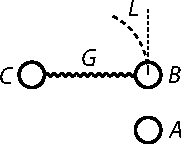
\includegraphics[width=0.20\textwidth]{gesamttex/edit_VIII-4/images/LH_35_11_14_005-006_d08_006r.pdf}%
\edcaption[0.50em]%
{%
\hspace{-95mm}%
\lbrack\textit{Fig.\:8}\rbrack%
\edtext{}{\lemma{\lbrack\textit{Fig.\:8}\rbrack}%
\Cfootnote[nonum]{%
Der Kreisbogen \textit{BL} fehlt in Leibnizens Zeichnung.%
}}%
}%
\vspace{-8.25em}%
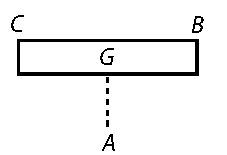
\includegraphics[width=0.25\textwidth]{gesamttex/edit_VIII-4/images/LH_35_11_14_005-006_d09_006r.pdf}%
\edcaption[0.25em]%
{%
\lbrack\textit{Fig.\:9}\rbrack%
}%
\vspace{-8.50em}%
\hspace{95mm}%
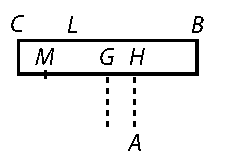
\includegraphics[width=0.25\textwidth]{gesamttex/edit_VIII-4/images/LH_35_11_14_005-006_d10_006r.pdf}%
\edcaption[0.25em]%
{%
\hspace{95mm}%
\lbrack\textit{Fig.\:10}\rbrack%
}%
\end{edfigure}%
\newpage%
\pstart%
Et quidem considerandum est%
\lbrack:\rbrack\
cum ictus%
\indexS{ictus eccentricus}
impellentis \textit{A}%
\indexS{corpus impellens}
non dirigitur in \textit{G} %
\edtext{sed
\edtext{in \textit{H},}{%
\lemma{in \textit{H}}\Cfootnote{%
Vgl. das Diagramm \lbrack\textit{Fig.\:10}\rbrack.}}
tunc totius \textit{BC} %
partem centrice ab \textit{A} in \textit{H} impulsam,%
\indexS{pars impulsa centrice}%
\indexS{impulsus centricus}
esse \lbrack\textit{BL}\rbrack,
residuumque %
tantum per consequentiam impulsum esse.%
\indexS{pars impulsa per consequentiam}
Et si \textit{CL} sit infinite parvum %
adeoque \textit{H} et \textit{G} coincidant,
tunc%
}{%
\lemma{sed}\Bfootnote{%
in \textit{H}
\textit{(1)}~tunc si \textit{H} et \textit{G} concidant seu si
\textit{(2)}~tunc totius %
\lbrack...\rbrack\ impulsam, esse 
\bars{\textit{BC}, \textit{ändert Hrsg.}}
residuumque, tantum
\lbrack...\rbrack\ coincidant, tunc%
~\textit{L}}}
cessare gyrum,%
\indexS{gyrus post ictum}
ob inconsiderabilem resistentiam ipsius \textit{CL}.%
\indexS{resistentia inconsiderabilis}
Sed quo major sit \textit{CL},
eo plus virium impendi in gyrum.
An ergo partibus \textit{BL} et \textit{CL}
positis aequalibus media pars in gyrum,%
\indexS{vis impensa in gyrum}
altera in communem progressum%
\indexS{vis impensa in progressum}%
\indexS{progressus post ictum}
\edtext{impendetur.
An potius non tantum partes considerandae,
sed etiam distantia centrorum cujusque a centro \textit{G},%
\indexS{distantia a centro gravitatis}
seu \textit{LB} in \textit{GH}
an comparandum cum \textit{CL} in \textit{MG}.
Sed video id fieri non debere.%
}{%
\lemma{impendetur.}\Bfootnote{%
\textit{(1)}~An potius non ipsa
\textit{(2)}~Nam ut ipsarum
\textit{(3)}~An potius %
\lbrack...\rbrack\ etiam distantia
\textit{(a)}~earum centro
\textit{(b)}~centrorum cujusque a centro \textit{G},
\textit{(aa)}~sed si hoc
\textit{(bb)}~seu \textit{LB} %
\lbrack...\rbrack\ non debere.%
~\textit{L}}}
Nam ita in casu incursus in \textit{G},%
\indexS{incursus eccentricus}
si \textit{H} et \textit{G} coinciderent,
tamen aequale foret factum \textit{LB} in \textit{HG} infinite parvum,
et infinite parvum \textit{CL} in ordinarium \textit{HM}.
\lbrack%
\href{\Scan{LH_35_11_14_006v}}%
{6\,v\textsuperscript{o}}%
\rbrack\ %
Et sane nec apparet
quid in propulsione totius \textit{CB}%
\indexS{propulsio}
prospectus centri \textit{G} conferat.%
\indexS{prospectus}
An
\edtext{rem concipiemus}{%
\lemma{rem}\Bfootnote{%
\textit{(1)}~sit
\textit{(2)}~concipiemus%
~\textit{L}}}
\edtext{methodo alibi feliciter adhibita%
\indexS{methodus feliciter adhibita}%
}{%
\lemma{methodo \lbrack...\rbrack\ adhibita}%
\Cfootnote{Gemeint ist wohl die \textit{methodus alternorum seu elective concurrentium}, die Leibniz bereits einige Jahre zuvor (1686 \textendash\ Oktober 1687) auf den schiefen Stoß angewandt hatte
(siehe \cite{01398}%
\textit{LSB} VIII,\;3 N.\;65\textsubscript{2}). %
Diese Methode hatte er in der
\cite{01098}%
\textit{Demonstratio geometrica regulae apud Staticos receptae} mathematisch nachgewiesen
(\textit{AE} November 1685, S.\;501--505;\cite{01023}
N.\;\ref{49409} im vorliegenden Band).%
}}%
\lbrack,\rbrack\
ut utrumque ponamus integre succedere
quasi duplicato corpore,
et
\edtext{deinde medium
(\protect\vphantom)%
sed justitiae%
\indexS{justitia}%
\protect\vphantom()
eligamus.%
}{%
\lemma{deinde}\Bfootnote{%
\textit{(1)}~centri gravitatis
\textit{(2)}~medium
\bars{et gyrum \textit{gestr.}}
(\protect\vphantom)sed justitiae\protect\vphantom() eligamus.%
~\textit{L}}}
Quod quomodo hic reperiri possit
dispiciendum.
\pend%
\vspace*{2.5em}%
\centerline{%
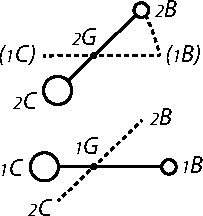
\includegraphics[width=0.24\textwidth]{gesamttex/edit_VIII-4/images/LH_35_11_14_005-006_d11_006v.pdf}}%
\vspace{0.25em}%
\centerline{%
\lbrack\textit{Fig.\:11}\rbrack}%
\newpage%
\pstart%
Sit igitur velocitas ut 1%
\indexS{velocitas distribuenda inter gyrum et progressum}
distribuenda inter gyrum%
\indexS{gyrus post ictum}
\edtext{circa \textit{G}}{%
\lemma{circa \textit{G}}\Cfootnote{%
Vgl. das Diagramm \lbrack\textit{Fig.\:11}\rbrack.}}
et progressum \textit{\ind{1}G\ind{2}G}.%
\indexS{progressus post ictum}
\edtext{Ponamus totam primo impendi in progressum,%
\indexS{veloctias impensa in progressum}%
}{%
\lemma{Ponamus}\Bfootnote{%
\textit{(1)}~totum progress
\textit{(2)}~totam primo impendi in progressum,%
~\textit{L}}}
seu esse
$\ind{1}G\ind{2}G = 1,$
et quantitas progressus erit%
\indexS{quantitas progressus}
\edlabel{LH_35_11_14_006v_qvmh-1}%
\edtext{}{%
\xxref{LH_35_11_14_006v_qvmh-1}{LH_35_11_14_006v_qvmh-2}%
\lemma{\ind{1}G\ind{2}G in $B + C$}\Cfootnote{%
Zu lesen wie $\ind{1}G\ind{2}G \cdot (B + C).$
Klammern werden bei den folgenden Rechnungen zumeist nicht berücksichtigt.%
}}%
\textit{\ind{1}G\ind{2}G} in
\edtext{$B + C.$%
\edlabel{LH_35_11_14_006v_qvmh-2}
Sin omnis vis impendatur in gyrum,%
\indexS{vis impensa in gyrum}
fiet}{\lemma{$B + C$}\Bfootnote{%
\textit{(1)}~, restat
\textit{(2)}~. Sin omnis %
\lbrack...\rbrack\ gyrum, fiet%
~\textit{L}}}
\textit{\ind{1}C\ind{2}C} in $C
+
\ind{1}B\ind{2}B$ in $B
=
\ind{1}G\ind{2}G$ in $B + C.$
Est autem
\textit{\ind{1}C\ind{2}C} ad
\textit{\ind{1}B\ind{2}B}
ut \textit{B} ad \textit{C},
seu
$\ind{1}C\ind{2}C =
\ind{1}B\ind{2}B \cdot B : C$.
Ergo fiet continuo
$\ind{1}B\ind{2}B \cdot B +
\ind{1}B\ind{2}B \cdot B =
\ind{1}G\ind{2}G$
in $B + C.$
Ergo fieret
$\ind{1}B\ind{2}B =
\ind{1}G\ind{2}G,
B + C :
\edtext{[2]}{%
\lemma{2}\Bfootnote{%
\textit{erg. Hrsg.}}}
B.$
\pend%
\vspace{0.5em}%
\pstart%
\noindent%
\lbrack%
\textit{Nachfolgend kleingedruckter Text in L gestrichen:}\rbrack %
\pend%
\vspace{0.5em}%
\footnotesize%
\pstart%
\noindent%
Quod est absurdum,%
\indexS{absurdum}
nisi sint \textit{B} et \textit{C} aequales;
nam pari jure etiam \textit{\ind{1}C\ind{2}C} fieret
$\; =\ind{1}G\ind{2}G$
fierentque \textit{\ind{1}B\ind{2}B}
et \textit{\ind{1}C\ind{2}C} aequales inter se.
Unde jam videtur alia faciliore ratione
ex sola Hypothesi gyrationis%
\indexS{gyratio circa centrum gravitatis}%
\indexS{hypothesis}
circa centrum gravitatis%
\indexS{gyratio circa centrum gravitatis}
faciendae haberi exitus,%
\indexS{exitus}
quanta nempe pars motus%
\indexS{motus translatus in gyrum}
possit debeatve transferri in gyrum.%
\indexS{motus translatus in gyrum}%
\indexS{gyrus post ictum}
\edtext{Nam quaeritur}{%
\lemma{Nam}\Bfootnote{%
\textit{(1)}~sit
\textit{(2)}~quaeritur%
~\textit{L}}}
quae debeat esse proportio ipsius
$\ind{1}C\ind{2}C$
in \textit{C} et \textit{\ind{1}B\ind{2}B} in \textit{B},
\edtext{seu $\astrosun$}{%
\lemma{seu}\Bfootnote{%
$\astrosun$
\textit{erg.\;L}}}
ad \textit{\ind{1}G\ind{2}G} in $B + C$
\edtext{seu $\rightmoon.$}{%
\lemma{seu}\Bfootnote{%
$\rightmoon$
\textit{erg.\;L}}}
Cum sit
\textit{\ind{1}C\ind{2}C}
ad \textit{\ind{1}B\ind{2}B} %
ut \textit{B} ad \textit{C},
fiet
$\ind{1}C\ind{2}C =
\ind{1}B\ind{2}B \cdot B : C$
seu
\textit{\ind{1}C\ind{2}C} in
$C = \ind{1}B\ind{2}B$ in \textit{B},
\edtext{et $\astrosun =
\ind{1}C\ind{2}C +
\ind{1}B\ind{2}B$
in \textit{B} erit%
}{%
\lemma{et}\Bfootnote{%
\textit{(1)}~fit ratio
\textit{(2)}~$\astrosun = \ind{1}C\ind{2}C$ in $C + \ind{1}B\ind{2}B$ in \textit{B} erit%
~\textit{L}}} 
$=\;\ind{1}B\ind{2}B$
in \textit{B}\,bis%
\lbrack,\rbrack\
posito $\astrosun$
\edtext{esse quantitatem vis respectivae%
\indexS{vis respectiva}%
}{\lemma{esse}\Bfootnote{%
\textit{(1)}~vim i
\textit{(2)}~quantitatem
\textit{(a)}~motus progressus
\textit{(b)}~vis respectivae%
~\textit{L}}}
impendendam in%
\indexS{vis impensa in gyrum}
\edtext{gyrum%
\indexS{gyrus post ictum}
et $\rightmoon$ esse quantitatem vis respectivae%
\indexS{vis respectiva}
impendendam in progressum totalem.%
\indexS{vis impensa in progressum}
Ergo fit%
}{%
\lemma{gyrum}\Bfootnote{%
\textit{(1)}~. Ergo fit
\textit{(2)}~et $\rightmoon$ \lbrack...\rbrack\ Ergo fit %
~\textit{L}}}
$\astrosun$ ad $\rightmoon$
ut \textit{\ind{1}B\ind{2}B} in \textit{B}\,bis
ad \textit{\ind{1}G\ind{2}G} in $B + C$
seu in ratione composita \textit{\ind{1}B\ind{2}B}
ad \textit{\ind{1}G\ind{2}G} %
et $B + C$ ad \textit{\ind{2}B},
vel in ratione composita \textit{\ind{1}C\ind{2}C}
ad \textit{\ind{1}G\ind{2}G} %
et $B + C$
\edtext{ad \textit{C}.
Habemus ergo $\astrosun = \ind{1}B\ind{2}B \cdot 2B$%
}{%
\lemma{ad}\Bfootnote{%
\textit{C}.
\textit{(1)}~Sed
\textit{(2)}~Habemus ergo
\textit{(a)}~$\ind{1}B\ind{2}B = \ind{1}G\ind{2}G \cdot \ind{1}B\ind{2}B : B$
\textit{(b)}~$\astrosun \cdot \ind{1}B\ind{2}B$
\textit{(c)}~$\astrosun = \ind{1}B\ind{2}B\cdot2B$%
~\textit{L}}}
et $\rightmoon$
{\normalsize%
\lbrack\textit{Text bricht ab.}\rbrack}%
\pend%
\vspace{0.65em}%
\normalsize%
\pstart%
\noindent%
Unde sequitur
\textit{B} moveri in linea spirali%
\indexS{linea spiralis}%
\indexS{spiralis}
composita ex circulatione%
\indexS{circulatio circa centrum gravitatis}
\edtext{circa \textit{G}}{%
\lemma{circa}\Bfootnote{%
\textit{G}
\textit{erg.\;L}}}
et progressu,%
\indexS{progressus in concursu eccentrico}
ut et \textit{C} in alia spirali data moveri.%
\indexS{spiralis}
Verum alia fit spiralis ipsius \textit{B} %
(\protect\vphantom)%
adeoque et ipsius\;\textit{C}%
\lbrack\protect\vphantom()\rbrack\
si minor impendenda sit pars in gyrum,%
\indexS{vis impensa in gyrum}
quam in progressum,%
\indexS{vis impensa in progressum}
vel si major.
Quid si ergo omnes spirales ponamus%
\indexS{spiralis}
\edtext{%
describi a puncto \textit{B} singulatim;
sed quaeritur quae ex ipsis eligi debeat%
}{%
\lemma{describi}\Bfootnote{%
\textit{(1)}~eligamusque
\textit{(2)}~a puncto %
\lbrack...\rbrack\ eligi debeat%
~\textit{L}}}%
\lbrack,\rbrack\
nempe alia debet eligi
prout alia est proportio ipsius \textit{B} ad \textit{C}.
Quid si ponamus \textit{B} majorem ipsa \textit{C},
divulsam intelligi in duas partes,
unam aequalem ipsi \textit{C},
quae medietatem accipiat gyri,%
\indexS{gyrus post ictum}
medietatem habeat progressus,%
\indexS{progressus post ictum}
altera quae sit excessus\;\textit{B} supra \textit{C},
ob
\edtext{quam progressus excedit gyrum%
\indexS{progressus excedens gyrum}%
\lbrack?\rbrack\
Sed nondum apparet,
quomodo inde instituatur rationcinatio.%
\indexS{ratiocinatio}
An hoc modo%
\lbrack:\rbrack\
ipsius \textit{B} partes sint duae%
\lbrack,\rbrack\
una \textit{M} aequalis ipsi\;\textit{C},
altera \textit{L}.
Iam \textit{M} et\;\textit{C} moventur in linea spirali,%
\indexS{linea spiralis}%
\indexS{spiralis}
ubi motus gyrationis%
\indexS{motus gyrationis}%
\indexS{gyratio circa centrum gravitatis}
et progressus sint inaequales,%
\indexS{motus progressus}
\textit{L} vero moveatur in sola recta.%
}{%
\lemma{quam}\Bfootnote{%
\textit{(1)}~\textlangle non\textrangle\ progressus
\textit{(2)}~progressus excedit gyrum
\textit{(a)}~, itaque ponamus
\textit{(aa)}~celerita
\textit{(bb)}~\textit{L} progredi ea celeritate qua centrum gravitatis \textit{G} ad \textit{C}
\textit{(aaa)}~per
\textit{(bbb)}~et partem ipsius \textit{B} ipsi aequalem circulari aequa
\textit{(b)}~. Sed nondum %
\lbrack...\rbrack\ hoc modo
\textit{(aa)}~ut
\textit{(bb)}~sit
\textit{(cc)}~p\textlangle\textendash\textrangle\
\textit{(dd)}~ipsius \textit{B} %
\lbrack...\rbrack\ duae una
\textit{(aaa)}~\textlangle$D = C$\textrangle\
\textit{(bbb)}~\textit{M} aequalis %
\lbrack...\rbrack\ sint inaequales,
\textit{(aaaa)}~sed \textlangle in una recta\textrangle\
\textit{(bbbb)}~\textit{L}
\bars{vero \textit{erg.}}
moveatur in sola recta.%
~\textit{L}}}
\edtext{%
Sed nihil
\edtext{inde.
Itaque
\edtext{a signo NB paginae praecedentis}{%
\lemma{a signo \lbrack...\rbrack\ praecedentis}\Cfootnote{%
Vgl. \refpassage{LH_35_11_14_006r_NBNB-1}{LH_35_11_14_006r_NBNB-2}.}}
nondum profecimus.%
}{%
\lemma{inde.}\Bfootnote{%
\textit{(1)}~An ita? \textit{B} progrediatur
\textit{(2)}~Itaque
\bars{inde \textit{streicht Hrsg.}}
a signo %
\lbrack...\rbrack\ nondum profecimus.%
~\textit{L}}}%
}{%
\lemma{\textit{Am Rand:}}\Afootnote{%
Nihil actum inter duo NB,
paginae%
\indexS{pagina}
scil. praecedentis%
\textsuperscript{\lbrack a\rbrack}
et hujus.%
\textsuperscript{\lbrack b\rbrack}%
\\[1ex]%
{\footnotesize%
\textsuperscript{\lbrack a\rbrack}~paginae scil. praecedentis:
\refpassage{LH_35_11_14_006r_NBNB-1}{LH_35_11_14_006r_NBNB-2}.
\quad%
\textsuperscript{\lbrack b\rbrack}~hujus:
\refpassage{LH_35_11_14_006v_NBNB-1}{LH_35_11_14_006v_NBNB-2}.%
}}}%
\pend%
\begin{edfigure}[0.00em][1.50em]%
\vspace*{7.00em}%
\hspace{-75mm}%
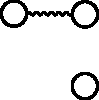
\includegraphics[width=0.11\textwidth]{gesamttex/edit_VIII-4/images/LH_35_11_14_005-006_d12_006v.pdf}%
\edcaption[0.50em]%
{%
\hspace{-75mm}%
\lbrack\textit{Fig.\:12}\rbrack%
}%
\vspace{-12.85em}%
\hspace{55mm}%
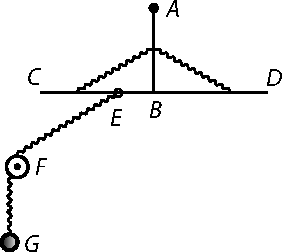
\includegraphics[width=0.34\textwidth]{gesamttex/edit_VIII-4/images/LH_35_11_14_005-006_d13_006v.pdf}%
\edcaption[-0.5em]%
{%
\hspace{58mm}%
\lbrack\textit{Fig.\:13}\rbrack%
\edtext{}{%
\lemma{\textit{Unter} \lbrack\textit{Fig.\:13}\rbrack\ \textit{und hierauf bezogen:}}%
\Afootnote[nonum]{%
Quid si flatus%
\indexS{flatus}
aliquis fiet lineis horizontalibus%
\textsuperscript{\lbrack a\rbrack}
normalibus in \textit{CD},
occupantibus exiguum circulum circa \textit{E}.
Quaeritur
an nulla fiat elevatio,%
\indexS{elevatio}
sed sola circulatio.%
\indexS{circulatio in tractione}
Puto utrumque.%
\\[1ex]%
{\footnotesize%
\textsuperscript{\lbrack a\rbrack}~horizontalibus
\textit{(1)}~aequalibus in punctum \textit{C}
\textit{(2)}~normalibus in \textit{CD},%
~\textit{L}%
}}}%
}%
\end{edfigure}%
\pstart%
Videamus an aliquis detur exitus,%
\indexS{exitus}
supponendo non tantum \textit{A} et \textit{G}
(\protect\vphantom)%
centrum gr. \textit{B} et \textit{C}%
\lbrack\protect\vphantom()\rbrack,
sed etiam \textit{C} et centrum gr.%
\indexS{centrum gravitatis commune}
inter \textit{A} et \textit{B} eandem servare vim%
\indexS{vis respectiva}
\edtext{respectivam.%
\edtext{\textls{ }%
\edlabel{LH_35_11_14_006v_NBNB-1}%
\textls{NB}%
\edlabel{LH_35_11_14_006v_NBNB-2}%
}{\lemma{\textit{Am Rand:}}\Afootnote{%
\textls{NB NB }%
}}\textls{ }%
Si
\edtext{ex funiculo \textit{AB}%
\indexS{funiculum}%
}{%
\lemma{ex funiculo \textit{AB}}\Cfootnote{%
Vgl. das Diagramm \lbrack\textit{Fig.\:13}\rbrack.%
}}%
}{%
\lemma{respectivam.}\Bfootnote{%
\bars{Imo res jam ex sola gyratione ipsius \textit{A} et \textit{G} fortassis determinata, jam enim constat, qua celeritate reflecti debeat \textit{A}, ea scil. quae sit dimidia vis respectivae. \textit{gestr.}}
\bars{\textls{NB} \textit{erg.}}
\textit{(1)}~Si sine ictu
\textit{(2)}~Si ex funiculo \textit{AB}%
~\textit{L}}}
suspendas trabem horizontalem \textit{CD},%
\indexS{trabs horizontalis}
inde
\edtext{alligato fune \textit{FE} ad \textit{CD},%
\indexS{funis trahens}
si placet %
normali,
in puncto \textit{E} extra medium trabis,}{%
\lemma{alligato \lbrack...\rbrack\ trabis}\Cfootnote{%
Anders als im Text angegeben,
verläuft das Seil \textit{EF} im Diagramm \lbrack\textit{Fig.\:13}\rbrack\ nicht senkrecht zum Balken \textit{CD}, sondern schräg hierzu.%
}}
trahas trabem,%
\indexS{trabs tracta}
potest ea duobus modis accedere
\edtext{ad \textit{F},
uno}{%
\lemma{ad}\Bfootnote{%
\textit{(1)}~trabem, uno
\textit{(2)}~\textit{F}, uno%
~\textit{L}}}
ut \textit{C\,E\,B\,D}
\edtext{parallel\lbrack e\rbrack}{%
\lemma{parallelae}\Bfootnote{%
\textit{L~ändert Hrsg.}}}
accedant,
altero
ut fiat gyratio%
\indexS{gyratio in tractione}
circa aliquod punctum, ut \textit{B}.
Quaeritur
quomodo fiat motus:
Haud dubie
\edtext{sic,
ut eodem manente descensu}{%
\lemma{sic,}\Bfootnote{%
ut
\textit{(1)}~ascensu
\textit{(2)}~eodem manente descensu%
~\textit{L}}}
ipsius \textit{G} ponderis,%
\indexS{descensus ponderis}
sit ascensus centri gravitatis trabis \textit{B}%
\indexS{ascensus centri gravitatis}%
\indexS{centrum gravitatis trabis}%
\indexS{trabs horizontalis}
omnium possibilium minimus.
Quanquam et
\edtext{si\lbrack c\rbrack}{%
\lemma{si}\Bfootnote{%
\textit{L~ändert Hrsg.}}}
decidatur%
\lbrack,\rbrack\
fateor ex eo non decidi nostrum,
habet tamen cum eo similitudinem.%
\indexS{similitudo}
\edtext{Nam hic}{%
\lemma{Nam}\Bfootnote{%
\textit{(1)}~si loco funis
\textit{(2)}~hic%
~\textit{L}}}
ponitur nulla opus vi
\edtext{ad circumagendam trabem,%
\indexS{trabs circumagenda}
quia solo conatu,%
\indexS{conatus sine impetu}
non impetu agitur,%
\indexS{impetus}
sed}{%
\lemma{ad}\Bfootnote{%
\textit{(1)}~circumagendum funiculum
\textit{(2)}~circumagendam trabem,
\textit{(a)}~\bars{\textlangle sed\textrangle\ \textit{streicht Hrsg.}}
\textit{(b)}~quia solo %
\lbrack...\rbrack\ agitur, sed%
~\textit{L}}}
ad \textit{A} circumagendum cum impulsu%
\indexS{impulsus}
est opus vi seu impetu,%
\indexS{impetus}%
\indexS{vis seu impetus}
si scilicet aliquod
\edtext{pondus in \textit{E} incidat.%
\indexS{pondus incidens}%
}{%
\lemma{pondus}\Bfootnote{%
\textit{(1)}~in \textlangle \textit{B} in\textrangle\ 
\textit{(2)}~in \textit{E} incidat.%
~\textit{L}}}
Ubi quidem talis orietur progressus,%
\indexS{progressus post concursum}
reflexio%
\indexS{reflexio post concursum}
et gyratio%
\indexS{gyratio post concursum}
ut eadem sit potentia%
\indexS{potentia post concursum}
quae ante concursum,%
\indexS{potentia ante concursum}
deinde etiam
ut eadem sit progressio centri gravitatis%
\indexS{progressio centri gravitatis}
quae ante concursum%
\indexS{concursus corporum}
si omnia subito lineis rigidis connectantur,%
\indexS{linea rigida}%
\indexS{corpora connexa}
postremo eadem vis respectiva,%
\indexS{vis respectiva}
intendens lineas connectentes.%
\indexS{linea connectens}
Sed haec non videntur sufficere ad determinandum.
Pono corpus in \textit{E} incurrens rigide,%
\indexS{corpus incurrens rigide}%
\indexS{incursus rigidus}
ipsi \textit{E} annecti
ut non possit dissilire.
Omnis vis respectiva non videtur hic perire%
\indexS{vis respectiva}%
\indexS{vis periens}
alligatione in \textit{E}.%
\indexS{alligatio}
Si enim pondus impingens in \textit{E}%
\indexS{pondus impingens}
et \textit{CD} in diversa tendunt%
\lbrack,\rbrack\
adjuvat \textit{BD} ipsum \textit{E} contra \textit{BC},
ut fiat gyratio%
\indexS{gyratio in tractione}
v.\,g. circa \textit{B}.
Si igitur \textit{CD} et pondus ut
\edtext{\lbrack\textit{G}\rbrack}{%
\lemma{\textit{F}}\Bfootnote{%
\textit{L~ändert Hrsg.}}}
funem \textit{FE} in diversa trahant%
\indexS{tractio funis}%
\lbrack,\rbrack\
quaeritur quantum intendatur funis,%
\indexS{funis tractus}%
\indexS{funis intensus}
quantum gyrationis,%
\indexS{gyratio in tractione}
quae minima mutatio,%
\indexS{mutatio minima}
et quae quantitas aestimanda.%
\indexS{quantitas aestinamda}%
\pend%
\selectlanguage{latin}%
\frenchspacing%
\normalsize%
